%!TEX platex=1
\documentclass[11pt,xcolor=dvipsnames,table,dvipdfmx]{beamer}
\usepackage{amsmath, amssymb}
\usepackage{latexsym}
\usepackage{ascmac}
\usepackage{bm}

%Beamer$B$N@_Dj(B
\usetheme{Boadilla}
%Beamer$B%U%)%s%H@_Dj(B
\usepackage{txfonts} % TX$B%U%)%s%H(B
\usepackage[deluxe]{otf} % $BF|K\8lB?%&%'%$%H2=(B
\renewcommand{\familydefault}{\sfdefault}  % $B1QJ8$r%5%s%;%j%UBN$K(B
\renewcommand{\kanjifamilydefault}{\gtdefault}  % $BF|K\8l$r%4%7%C%/BN$K(B
\usefonttheme{professionalfonts}
\setbeamerfont{alerted text}{series=\bfseries} % Alert$B$rB@;z(B
\setbeamerfont{section in toc}{series=\mdseries} % $BL\<!$OB@;z$K$7$J$$(B
\setbeamerfont{frametitle}{size=\Large} % $B%U%l!<%`%?%$%H%kJ8;z%5%$%:(B
\setbeamerfont{title}{size=\LARGE} % $B%?%$%H%kJ8;z%5%$%:(B
\setbeamerfont{date}{size=\small}  % $BF|IUJ8;z%5%$%:(B

%Beamer$B?'@_Dj(B
\definecolor{UniBlue}{RGB}{0,150,200} 
\definecolor{AlertOrange}{RGB}{255,76,0}
\definecolor{AlmostBlack}{RGB}{38,38,38}
\setbeamercolor{normal text}{fg=AlmostBlack}  % $BK\J8%+%i!<(B
\setbeamercolor{structure}{fg=UniBlue} % $B8+=P$7%+%i!<(B
\setbeamercolor{block title}{fg=UniBlue!50!black} % $B%V%m%C%/ItJ,%?%$%H%k%+%i!<(B
\setbeamercolor{alerted text}{fg=AlertOrange} % \alert $BJ8;z%+%i!<(B
\mode<beamer>{
    \definecolor{BackGroundGray}{RGB}{254,254,254}
    \setbeamercolor{background canvas}{bg=BackGroundGray} % $B%9%i%$%I%b!<%I$N$_GX7J$r$o$:$+$K%0%l!<$K$9$k(B
}

%$B%U%i%C%H%G%6%$%s2=(B
\setbeamertemplate{blocks}[rounded] % Block$B$N1F$r>C$9(B
\useinnertheme{circles} % $B2U>r=q$-$r%7%s%W%k$K(B
\setbeamertemplate{navigation symbols}{} % $B%J%S%2!<%7%g%s%7%s%\%k$r>C$9(B
\setbeamertemplate{footline}[frame number] % $B%U%C%?!<$O%9%i%$%IHV9f$N$_(B

%$B%?%$%H%k%Z!<%8(B
\setbeamertemplate{title page}{%
    \vspace{2.5em}
    {\usebeamerfont{title} \usebeamercolor[fg]{title} \inserttitle \par}
    {\usebeamerfont{subtitle}\usebeamercolor[fg]{subtitle}\insertsubtitle \par}
    \vspace{1.5em}
    \begin{flushright}
        \usebeamerfont{author}\insertauthor\par
        \usebeamerfont{institute}\insertinstitute \par
        \vspace{3em}
        \usebeamerfont{date}\insertdate\par
        \usebeamercolor[fg]{titlegraphic}\inserttitlegraphic
    \end{flushright}
}

% graphicx.sty
\usepackage{graphicx}

%
\def\qed{\hfill $\Box$}

\AtBeginSection[]{
    \frame{\tableofcontents[currentsection, hideallsubsections]} %$BL\<!%9%i%$%I(B
}

%$B%?%$%H%k(B
\title{Monthly Meeting on October}
\author{\textbf{Yuichiro Honda}}
\date{2016/11/02}
\institute{Morita lab. M1}

\begin{document}
\maketitle

\section{Previous work}
\begin{frame}{Last month}
 \begin{itemize}
  \item read a paper about an algorithm to find all common bases in two matroids in $O(n(n^2+t)\lambda)$
 \end{itemize}
\end{frame}

\section{Progress}
\begin{frame}{Matroid Intersection Problem}
 \begin{block}{Problem}
  input: \,\, $M_1 = (E, \mathcal{I}_1),\,\,M_2 = (E, \mathcal{I}_2)$ : matroids\\
  output: maximum-cardinality set $S \in \mathcal{I}_1 \cap \mathcal{I}_2$
 \end{block}
 note: Generally, $(E,\,\,\mathcal{I}_1 \cap \mathcal{I}_2)$ is not a matroid.
\end{frame}

\begin{frame}{Matroid Intersection Problem}
 \begin{block}{Lemma: unique perfect matching implies exchange}
  $M_1 := (E, \mathcal{I}): matroid$\\
  $S \in \mathcal{I},\,\,T \subset E$\\
  $S$
 \end{block}
 \begin{block}{Lemma: shortest implies augmenting}
  $M_1 := (E, \mathcal{I}_1),\,\, M_2 := (E, \mathcal{I}_2)$: matroid\\
  $S \in \mathcal{I}_1 \cap \mathcal{I}_2$\\
  If $P$ is a shortest source-sink dipath in $\mathcal{G}(S)$, then $P$ is augmenting path.
 \end{block}
\end{frame}

\begin{frame}{Matroid Intersection Problem}
 \begin{figure}
  \caption{$\mathcal{G}(S) := (S+E \setminus S,\,\, A)$ :bipartite graph}
  \centering
  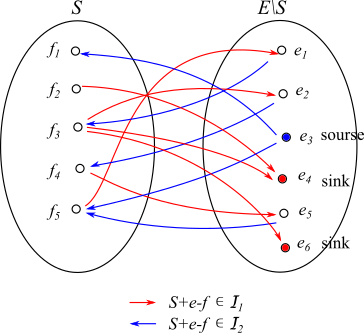
\includegraphics[width=6cm]{matching.png}\vspace{0.5cm}
 \end{figure}
\end{frame}

\begin{frame}{Matroid Intersection Problem}
 \begin{figure}
  \caption{source-sink dipath is augmenting path}
  \centering
  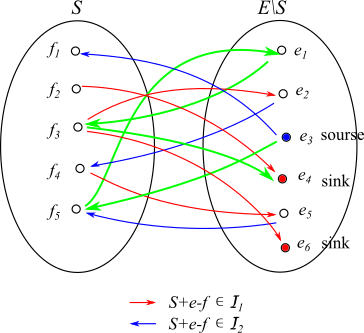
\includegraphics[width=6cm]{matching2.png}\vspace{0.5cm}
 \end{figure}
\end{frame}

\begin{frame}{Matroid Intersection Problem}
 \begin{block}{Matroid Intersection Algorithm}
  input: \,\, $M_1 = (E, \mathcal{I}_1),\,\,M_2 = (E, \mathcal{I}_2)$ : matroids\\
  output: maximum-cardinality set $S \in \mathcal{I}_1 \cap \mathcal{I}_2$
  \begin{enumerate}
   \item Start with $S \in \mathcal{I}_1 \cap \mathcal{I}_2$ such as $S := \emptyset $
   \item While $\mathcal{G}(S)$ has a source-sink dipath:\\
	 (1) $P := (e_0, f_1, e_1, ..., f_n, e_n)$ be an augmenting sequense\\
	 (2) $S := S \cup \{e_j |\,\,0 \leq j \leq n\} \setminus \{f_j |\,\,1 \leq j \leq n\}$
  \end{enumerate}
 \end{block}
 \begin{itemize}
  \item finding $P$ in $\mathcal{G}(S)$ requires $O(n^2)$\\
  \item  after step 2(2), regenerate $\mathcal{G}(S)$ requires $O(\tau n)$\\
 \end{itemize}
 $\rightarrow$ totally we have $O(\tau n^3)$ as time complexity
\end{frame}

\section{Next step}
\begin{frame}{next month}
 TODO:
 \begin{itemize}
  \item learn about alogrithm for finding k-best perfect matching
 \end{itemize}
\end{frame}

\section{Reference}
\begin{frame}{Reference}
 \begin{thebibliography}{9}
  \bibitem{1}
	  \small{Jon Lee: ``A First Course in Combinatorial Optimization''}
 \end{thebibliography}
\end{frame}

\end{document}